\documentclass{beamer}
\mode<presentation> {
% The Beamer class comes with a number of default slide themes
% which change the colors and layouts of slides. Below this is a list
% of all the themes, uncomment each in turn to see what they look like.
\usepackage{diagbox}
\usepackage{makecell}
%\usetheme{default}
%\usetheme{AnnArbor}
%\usetheme{Antibes}
%\usetheme{Bergen}
%\usetheme{Berkeley}
%\usetheme{Berlin}
%\usetheme{Boadilla}
%\usetheme{CambridgeUS}
%\usetheme{Copenhagen}
%\usetheme{Darmstadt}
%\usetheme{Dresden}
%\usetheme{Frankfurt}
%\usetheme{Goettingen}
%\usetheme{Hannover}
%\usetheme{Ilmenau}
%\usetheme{JuanLesPins}
%\usetheme{Luebeck}
\usetheme{Madrid}
%\usetheme{Malmoe}
%\usetheme{Marburg}
%\usetheme{Montpellier}
%\usetheme{PaloAlto}
%\usetheme{Pittsburgh}
%\usetheme{Rochester}
%\usetheme{Singapore}
%\usetheme{Szeged}
%\usetheme{Warsaw}
\usepackage{tabularx,multirow,booktabs}
\usepackage{ragged2e}
\usepackage{stackengine}
\usepackage{algorithm}
\usepackage[noend]{algpseudocode}
%\usepackage{bibentry}
\usepackage{biblatex}
\addbibresource{sample.bib}
% As well as themes, the Beamer class has a number of color themes
% for any slide theme. Uncomment each of these in turn to see how it
% changes the colors of your current slide theme.

%\usecolortheme{albatross}
%\usecolortheme{beaver}
%\usecolortheme{beetle}
%\usecolortheme{crane}
%\usecolortheme{dolphin}
%\usecolortheme{dove}
%\usecolortheme{fly}
%\usecolortheme{lily}
%\usecolortheme{orchid}
%\usecolortheme{rose}
%\usecolortheme{seagull}
%\usecolortheme{seahorse}
%\usecolortheme{whale}
%\usecolortheme{wolverine}

\setbeamertemplate{bibliography item}[triangle]
\setbeamertemplate{caption}{\insertcaption}
\setbeamertemplate{footline}
{
	\leavevmode%
	\hbox{%
		\begin{beamercolorbox}[wd=.333333\paperwidth,ht=2.25ex,dp=1ex,center]{author in head/foot}%
			\usebeamerfont{author in head/foot}{George Joseph}
		\end{beamercolorbox}%
		\begin{beamercolorbox}[wd=.333333\paperwidth,ht=2.25ex,dp=1ex,center]{title in head/foot}%
			\usebeamerfont{title in head/foot}{SubGraph Isomorphism}
		\end{beamercolorbox}%
		\begin{beamercolorbox}[wd=.333333\paperwidth,ht=2.25ex,dp=1ex,right]{date in head/foot}%
			\usebeamerfont{date in head/foot}\insertshortdate{}\hspace*{2em}
			\insertframenumber{} \hspace*{2ex} 
		\end{beamercolorbox}}%
		\vskip0pt%
	}
	
%\setbeamertemplate{footline}{
%			\leavevmode%
%			\hbox{%
%				\begin{beamercolorbox}[wd=.4\paperwidth,ht=2.25ex,dp=1ex,center]{author in head/foot}%
%					\usebeamerfont{author in head/foot}\insertshortauthor
%				\end{beamercolorbox}%
%				\begin{beamercolorbox}[wd=.6\paperwidth,ht=2.25ex,dp=1ex,center]{title in head/foot}%
%					\usebeamerfont{title in head/foot}\insertshorttitle\hspace*{3em}
%					\insertframenumber{} / \inserttotalframenumber\hspace*{1ex}
%				\end{beamercolorbox}}%
%				\vskip0pt
%			} 
		
		% To remove the footer line in all slides uncomment this line
%\setbeamertemplate{footline}[page number] % To replace the footer line in all slides with a simple slide count uncomment this line

%\setbeamertemplate{navigation symbols}{} % To remove the navigation symbols from the bottom of all slides uncomment this line
}
\usepackage{graphicx} % Allows including images
\usepackage{booktabs} % Allows the use of \toprule, \midrule and \bottomrule in tables
\usepackage{multirow}
\usepackage{amsmath}
\usepackage{amsfonts}
\usepackage{multicol}
\usepackage[mathscr]{eucal}
\usepackage{graphics,tikz}
\usepackage {biblatex}
\usepackage{color}


%----------------------------------------------------------------------------------------
%	TITLE PAGE
%----------------------------------------------------------------------------------------
\makeatother
%\logo{\includegraphics[height=1.5cm]{IITM_emblum.jpg}}
\titlegraphic{\includegraphics[width=0.17\textwidth,height=.2\textheight]{IITM_emblum.jpg}}

\title[MLC]{Subgraph Isomorphism in GPU \\ } % The short title appears at the bottom of every slide, the full title is only on the title page

\author{{\fontsize{8}{6}\selectfont George Joseph (CS15M021) \\ \vspace{0.1cm}  \vspace{0.1cm} Guided by : Rupesh Nasre} } % Your name
\institute
{
% Under the guidance of \\ \vspace{0.1cm}
% Dr.C.Chandra Sekhar\\ % Your institution for the title page
\vspace{0.1cm}
\medskip
{\bf{Department of Computer Science and Engineering}}\\
{\bf{Indian Institute of Technology, Madras}}
}
 \date{\color{white}\today} % Date, can be changed to a custom date
\addbibresource{sample.bib}
\begin{document}	

	
	
\begin{frame}
\titlepage % Print the title page as the first slide

\end{frame}

\begin{frame}
\frametitle{Outline} % Table of contents slide, comment this block out to remove it
\tableofcontents

\end{frame}
\section{Motivation } 
\section{Problem Statement}
\section{Parallel Implementation}
\section{Experimental results}
\section{Dynamic Queries}
%----------------------------------------------------------------------------------------
%	PRESENTATION SLIDES
%----------------------------------------------------------------------------------------

%------------------------------------------------
\begin{frame}
\frametitle{Motivation}


    \begin{block}{Applications}
    \begin{itemize}
    \item Social Network
    \item Bio-Informatics
    \item Chemical Compound matching
    \item Pattern Recognition
    \end{itemize}
    \end{block}
    
  %  \item In web there are lots of unlabelled image data. Automatic image annotation is the best way to label it.
%\end{itemize}
%\end{frame}

%\begin{frame}
%\frametitle{Multi-Label learning for image annotation}
%\begin{itemize}

   % \begin{block}{Multi-Label learning}
    \begin{itemize}
      \item Subgraph Isomorphism Query is one of the most important graph queries.
    \end{itemize}
    %\end{block}
   % \begin{figure}
%    \centering
%    \includegraphics[width=0.3\textwidth, height = 2cm]{46030.jpeg}
%    \caption {Broad Category - Beach  \pause \color{red} Sand, mountain, sky, clouds}
   
%    \label{fig:my_label}
%\end{figure}


\end{frame}
\begin{frame}{Problem Statement}

\begin{block}{Input} A data Graph $D$, and Query Graph $Q$. The graphs $D$ and $Q$ are undirected with nodes and edges having label.
  \\
  Graphs given as adjacency list. 
  \\
  \end{block}
  \begin{block}{Output}
   Give all the matching mapping of each node in $Q$ to node in $D$ \\

\end{block}

    
\end{frame}
\begin{frame}{Example}
   \begin{figure}
	\begin{minipage}{.4\textwidth}
	\centering
	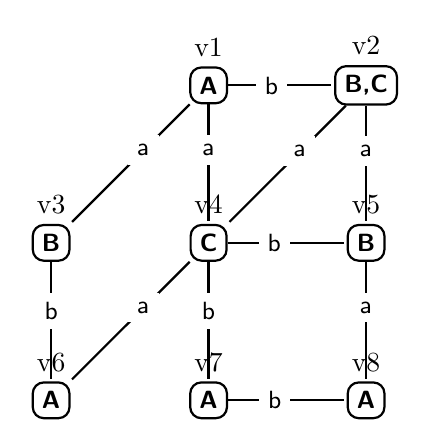
\begin{tikzpicture}[shorten >=1pt,auto,node distance=2cm,
                    thick,main node/.style={rounded corners,draw,font=\sffamily\small\bfseries}]

  \node[main node,label=v1] (1) {A};
  \node[main node,label=v2] (2) [right of=1] {B,C}; 
  \node[main node,label=v4] (4) [below of =1] {C};
  \node[main node,label=v3] (3) [left of=4] {B};
     \node[main node,label=v5] (5) [below of=2] {B};
    \node[main node,label=v6] (6) [below of=3] {A};
    \node[main node,label=v7] (7) [below of=4] {A};
\node[main node,label=v8] (8) [below of=5] {A};
  \path[every node/.style={font=\sffamily\small}]
    (1) edge[] node [minimum width = 1em, fill = white,pos=.25,right] {b} (2)
        edge[] node[minimum width = 1em, fill = white,pos=.25,below left] {a} (3)
        edge[] node[minimum width = 1em, fill = white,pos=.25,below] {a} (4)
    (2) edge[] node [minimum width = 1em, fill = white,pos=.25,below left] {a} (4)
        edge node [minimum width = 1em, fill = white,pos=.25,below] {a} (5)
    (3) edge[] node [minimum width = 1em, fill = white,pos=.25,below] {b} (6)
    (4) edge node [minimum width = 1em, fill = white,pos=.25,below] {b} (7)
    	edge[] node [minimum width = 1em, fill = white,pos=.25,below left] {a} (6) 
    	edge node [minimum width = 1em, fill = white,pos=.25,right] {b} (5) 
    (5) edge node [minimum width = 1em, fill = white,pos=.25,below] {a} (8)
    (7) edge node [minimum width = 1em, fill = white,pos=.25,right] {b} (8);	   
\end{tikzpicture}\\
Data Graph
\end{minipage}
\begin{minipage}{.4\textwidth}
\centering
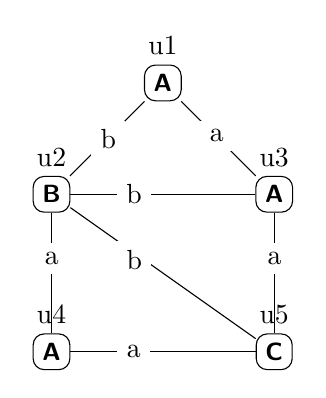
\begin{tikzpicture}[node distance=2cm,node/.style={rounded corners,draw,font=\sffamily\small\bfseries}]
	\node[node,label=u1] (1) {A};
	\node[node,label=u2] (2)[below left of=1] {B};
		\node[node,label=u3] (3)[below right of=1] {A};
		\node[node,label=u4] (4)[below  of=2] {A};
			\node[node,label=u5] (5)[below of=3] {C};
	\path
	(1) edge node [minimum width = 1em, fill = white,pos=.25,below left] {b} (2)
		edge node [minimum width = 1em, fill = white,pos=.25,below right]{a} (3)	
	(2) edge node [minimum width = 1em, fill = white,pos=.25,right]{b} (3)
		edge node [minimum width = 1em, fill = white,pos=.25,below]{a} (4)
		edge node [minimum width = 1em, fill = white,pos=.25,below right]{b} (5)
	(3) edge node [minimum width = 1em, fill = white,pos=.25,below]{a} (5)	
	(4) edge node [minimum width = 1em, fill = white,pos=.25,right]{a} (5);	
							
\end{tikzpicture}
\\ Query Graph
\end{minipage}
\caption{}
\end{figure}
\end{frame}
\begin{frame}{General Algorithm}
    %\begin{block}

    \begin{algorithm}[H]
    \caption{SubGraph Isomorphism}
    \textbf{Input: Query Graph (Q) and Data Graph(D)}
     \begin{enumerate}
           \item Find Candidates(CS) for each vertex in Q
          % \item Labels are divided into exclusive groups.
           % \item In each group we learn discriminative label specific dictionaries.
            \item Procedure SubgraphMatching
            \begin{enumerate}
                \item   if all vertices processed output the map
                \item u= NextVertex(Q)
                \item $C_r$= RefinedSet(CS,Q,D,v)
                \item for each v in $C_r$
                \begin{enumerate}
                    \item if IsJoinable(Q,D,M,v)
                    \item UpdateState(M,v)
                    \item Call SubgraphMatching
                    \item RestoreState(M,v)
                \end{enumerate}
            \end{enumerate}
        %    \item Relevant labels gets higher score than the irrelevant ones.
        \end{enumerate}
        \textbf{Output: Mappings M}
    \end{algorithm}
      
   % \end{block}
     
        % \item \color{blue} Multi-Label Dictionary Learning (MLDL) for Image Annotation
        % \begin{itemize}
    
        %   \item This method learns a single dictionary with label consistency regularization.
           
        %   \item This ensures discriminative sparse representation.
        %   \item Samples are transformed into a new space oriented by label information.
        %   \item A joint objective function for learning the dictionary and the transformation matrix.
        % \end{itemize}
\end{frame}




\begin{frame}
\frametitle{Candidate Vertex Set}

\begin{figure}
	\begin{minipage}{.4\textwidth}
	\centering
	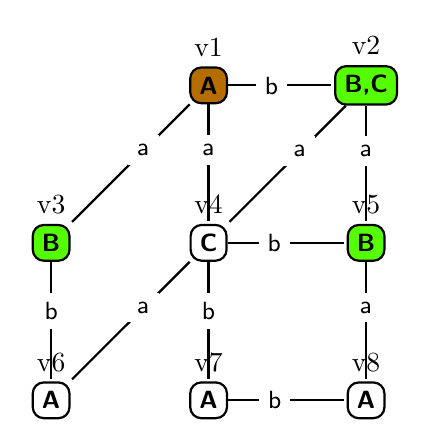
\begin{tikzpicture}[shorten >=1pt,auto,node distance=2cm,
                    thick,main node/.style={rounded corners,draw,font=\sffamily\small\bfseries}]

  \node[main node,fill={rgb:red,4;green,2;yellow,1},label=v1] (1) {A};
  \node[main node,fill={rgb:red,0;green,2;yellow,1},label=v2] (2) [right of=1] {B,C}; 
  \node[main node,label=v4] (4) [below of =1] {C};
  \node[main node,fill={rgb:red,0;green,2;yellow,1},label=v3] (3) [left of=4] {B};
     \node[main node,fill={rgb:red,0;green,2;yellow,1},label=v5] (5) [below of=2] {B};
    \node[main node,label=v6] (6) [below of=3] {A};
    \node[main node,label=v7] (7) [below of=4] {A};
\node[main node,label=v8] (8) [below of=5] {A};
  \path[every node/.style={font=\sffamily\small}]
    (1) edge[] node [minimum width = 1em, fill = white,pos=.25,right] {b} (2)
        edge[] node[minimum width = 1em, fill = white,pos=.25,below left] {a} (3)
        edge[] node[minimum width = 1em, fill = white,pos=.25,below] {a} (4)
    (2) edge[] node [minimum width = 1em, fill = white,pos=.25,below left] {a} (4)
        edge node [minimum width = 1em, fill = white,pos=.25,below] {a} (5)
    (3) edge[] node [minimum width = 1em, fill = white,pos=.25,below] {b} (6)
    (4) edge node [minimum width = 1em, fill = white,pos=.25,below] {b} (7)
    	edge[] node [minimum width = 1em, fill = white,pos=.25,below left] {a} (6) 
    	edge node [minimum width = 1em, fill = white,pos=.25,right] {b} (5) 
    (5) edge node [minimum width = 1em, fill = white,pos=.25,below] {a} (8)
    (7) edge node [minimum width = 1em, fill = white,pos=.25,right] {b} (8);	   
\end{tikzpicture}\\
Data Graph
\end{minipage}
\begin{minipage}{.4\textwidth}
\centering
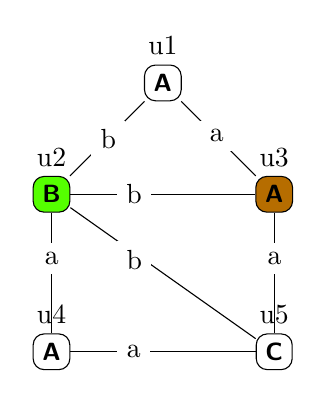
\begin{tikzpicture}[node distance=2cm,node/.style={rounded corners,draw,font=\sffamily\small\bfseries}]
	\node[node,label=u1] (1) {A};
	\node[node,fill={rgb:red,0;green,2;yellow,1},label=u2] (2)[below left of=1] {B};
		\node[node,fill={rgb:red,4;green,2;yellow,1},label=u3] (3)[below right of=1] {A};
		\node[node,label=u4] (4)[below  of=2] {A};
			\node[node,label=u5] (5)[below of=3] {C};
	\path
	(1) edge node [minimum width = 1em, fill = white,pos=.25,below left] {b} (2)
		edge node [minimum width = 1em, fill = white,pos=.25,below right]{a} (3)	
	(2) edge node [minimum width = 1em, fill = white,pos=.25,right]{b} (3)
		edge node [minimum width = 1em, fill = white,pos=.25,below]{a} (4)
		edge node [minimum width = 1em, fill = white,pos=.25,below right]{b} (5)
	(3) edge node [minimum width = 1em, fill = white,pos=.25,below]{a} (5)	
	(4) edge node [minimum width = 1em, fill = white,pos=.25,right]{a} (5);	
							
\end{tikzpicture}
\\ Query Graph
\end{minipage}
\caption{}
\end{figure}
\begin{itemize}
\item Based on Node Value
\item Based on Degree
\end{itemize}
\end{frame}

\begin{frame}
\frametitle{Sugbraph Matching}
\begin{block}{NextVertex}
\begin{itemize}
\item Order of processing query nodes
\item Taking u2 first gives a more refined search than taking any other node. 
\end{itemize}
\end{block}
\begin{block}{RefinedSet}
\begin{itemize}
\item Remove already mapped nodes
\item Once u3 is mapped v1 can be removed from CVS of u1.
\end{itemize}
\end{block}
\begin{block}{IsJoinable}
\begin{itemize}
\item Check existence of edges
\end{itemize}
\end{block}
\begin{block}{UpdateState and Restore State}
\begin{itemize}
\item Push and restore current mapped vertex
\end{itemize}
\end{block}
\end{frame}

%\begin{frame}
%\frametitle{Literature Survey:QuickSi}
%\begin{block}{RefinedSet}
%\begin{enumerate}
%    \item Connectivity to mapped vertices are checked
%\end{enumerate}
%\end{block}
%\begin{block}{NextVertex}
%    Takes the next most infrequent vertex.
%\end{block}
%\end{frame}
%
%\begin{frame}
%\frametitle{Literature Survey:VF2}
%\begin{block}{RefinedSet}
%\begin{enumerate}
%    \item Prune out v if not connected to already mapped vertices.
%    \item The count of neighbors of v who are neighbours of mapped nodes in $Q$ must be greater than neighbors of u who are neighbours of mapped nodes in $D$.
%    \item The count of neighbors of v who are not neighbours of mapped nodes and not mapped nodes in $Q$ must be greater than neighbors of u who are not neighbours of mapped nodes and not mapped nodes in $D$   
%\end{enumerate}
%\end{block}
%\begin{block}{NextVertex}
%    Takes the next connected vertex.
%\end{block}
%
%
%\end{frame}
%\begin{frame}{Literature Survey:GADDI}{Neighbourhood Discriminating Substructure}
%\begin{figure}
%	\begin{minipage}{.4\textwidth}
%	\centering
%	\begin{tikzpicture}[shorten >=1pt,auto,node distance=2cm,
%                    thick,main node/.style={rounded corners,draw,font=\sffamily\small\bfseries}]
%
%  \node[line width=1.6pt,main node,label=v1] (1) {A};
%  \node[line width=1.6pt,main node,label=v2] (2) [right of=1] {B,C}; 
%  \node[line width=1.6pt,main node,label=v4] (4) [below of =1] {C};
%  \node[line width=1.6pt,main node,label=v3] (3) [left of=4] {B};
%     \node[main node,label=v5] (5) [below of=2] {B};
%    \node[line width=1.6pt,main node,label=v6] (6) [below of=3] {A};
%    \node[main node,label=v7] (7) [below of=4] {A};
%\node[main node,label=v8] (8) [below of=5] {A};
%  \path[every node/.style={font=\sffamily\small}]
%    (1) edge[line width=.7mm] node [minimum width = 1em, fill = white,pos=.25,right] {b} (2)
%        edge[line width=.6mm] node[minimum width = 1em, fill = white,pos=.25,below left] {a} (3)
%        edge[line width=.65mm] node[minimum width = 1em, fill = white,pos=.25,below] {a} (4)
%    (2) edge[line width=.6mm] node [minimum width = 1em, fill = white,pos=.25,below left] {a} (4)
%        edge node [minimum width = 1em, fill = white,pos=.25,below] {a} (5)
%    (3) edge[line width=.65mm] node [minimum width = 1em, fill = white,pos=.25,below] {b} (6)
%    (4) edge node [minimum width = 1em, fill = white,pos=.25,below] {b} (7)
%    	edge[line width=.6mm] node [minimum width = 1em, fill = white,pos=.25,below left] {a} (6) 
%    	edge node [minimum width = 1em, fill = white,pos=.25,right] {b} (5) 
%    (5) edge node [minimum width = 1em, fill = white,pos=.25,below] {a} (8)
%    (7) edge node [minimum width = 1em, fill = white,pos=.25,right] {b} (8);	   
%\end{tikzpicture}\\
%$ \Delta_{NDS}(v1,v3,P1)=3    \Delta_{NDS}(v1,v3,P2)= 24  \Delta_{NDS}(v1,v3,P3)=12 $
%\end{minipage}
%\begin{minipage}{.45\textwidth}
%\centering
%\begin{tikzpicture}[node distance=1cm]
%\node[circle,draw] (1)[]{};
%\node[circle,draw] (2)[below left  of=1]{};
%\node[circle,draw] (3)[below right  of=1]{};
%\path
%	(1) edge node{} (2)
%		 edge node{} (3)
%	(2) edge node{} (3);	
%\end{tikzpicture}
%\\ P1\\ \hfill \\
%\begin{tikzpicture}[node distance=1cm]
%\node[circle,draw] (1)[]{};
%\node[circle,draw] (2)[right of=1]{};
%\node[circle,draw] (3)[right of=2]{};
%\node[circle,draw] (4)[right of=3]{};
%\path
%	(1) edge node{} (2)
%	(2) edge node{} (3)
%	(3) edge node{} (4);	
%\end{tikzpicture}
%\\ P2\\ \hfill \\
%\begin{tikzpicture}[node distance=1cm]
%\node[circle,draw] (4)[]{};
%\node[circle,draw] (1)[below of =4]{};
%\node[circle,draw] (2)[below left  of=1]{};
%\node[circle,draw] (3)[below right  of=1]{};
%
%\path
%	(1) edge node{} (2)
%		 edge node{} (3)
%	(4) edge node{} (1);	
%\end{tikzpicture}
%\\ P3
%\end{minipage}
%\caption{GADDI NDS Calculation}
%\end{figure}
%\end{frame}
%
%
%
%
%\begin{frame}{GADDI Cont..}
%
%    \begin{block}{RefinedSet}
%If for each $u^{'} \in N_{k}(u)$ there is no data vertex $v^{'} \in N_{k}(v)$ having
%	\begin{enumerate}
% \item $L(u^{'}) \subseteq L(v^{'})$ 
% \end{enumerate}
%\end{block}
%\end{frame}
%  
%
%  
%  \begin{frame}{GraphQL and SPath}
%\begin{figure}
%   \begin{minipage}{.6\textwidth}
%  \begin{block}{Neighbourhood Signature}
%  \begin{itemize}
%  \item GraphQL:one hop signature
%   \begin{itemize}
%  \item $ Sig(u1) = \{B,A\}$
%  \end{itemize}
%  \item SPath:k hop signature
%   \begin{itemize}
%  \item $ Sig(u1,2) = \{(1,B,1),(1,A,1),(2,A,1),(2.C,1)\}$
%  \end{itemize}
%  
%  \end{itemize}
% 
%  
%  \end{block}
%  \end{minipage}
%\begin{minipage}{.3\textwidth}
%\centering
%\begin{tikzpicture}[node distance=2cm,node/.style={rounded corners,draw,font=\sffamily\small\bfseries}]
%	\node[node,label=u1] (1) {A};
%	\node[node,label=u2] (2)[below left of=1] {B};
%		\node[node,label=u3] (3)[below right of=1] {A};
%		\node[node,label=u4] (4)[below  of=2] {A};
%			\node[node,label=u5] (5)[below of=3] {C};
%	\path
%	(1) edge node [minimum width = 1em, fill = white,pos=.25,below left] {b} (2)
%		edge node [minimum width = 1em, fill = white,pos=.25,below right]{a} (3)	
%	(2) edge node [minimum width = 1em, fill = white,pos=.25,right]{b} (3)
%		edge node [minimum width = 1em, fill = white,pos=.25,below]{a} (4)
%		edge node [minimum width = 1em, fill = white,pos=.25,below right]{b} (5)
%	(3) edge node [minimum width = 1em, fill = white,pos=.25,below]{a} (5)	
%	(4) edge node [minimum width = 1em, fill = white,pos=.25,right]{a} (5);	
%							
%\end{tikzpicture}
%\\ Query Graph
%\end{minipage}
% 
% 
% \end{figure}
%  \end{frame}
%
%\begin{frame}{STWig}
%    
%    \begin{itemize}
%       \item Query Graph Divided into small 2 level graphs
%       \item Each root in $j^{th}$ graph will be a child in a graph already created.
%       \item Each Subgraph Result is combined to get the final result
%    \end{itemize}
%    \begin{figure}[h]
% \centering
%%\centering
%\begin{minipage}{.3\textwidth}
%\begin{tikzpicture}[node distance=2cm]
%\node[circle,draw] (1)[]{A};
%\node[circle,draw] (2)[below left  of=1]{B};
%\node[circle,draw] (3)[below right  of=1]{A};
%\path
%	(1) edge node{} (2)
%		 edge node{} (3);	
%\end{tikzpicture}
%\end{minipage}
%\begin{minipage}{.3\textwidth}
%\begin{tikzpicture}[node distance=2cm]
%\node[circle,draw] (1)[]{B};
%\node[circle,draw] (2)[below left  of=1]{C};
%\node[circle,draw] (3)[below right  of=1]{A};
%\path
%	(1) edge node{} (2)
%		 edge node{} (3);	
%\end{tikzpicture}
%\end{minipage}
%\begin{minipage}{.3\textwidth}
%\begin{tikzpicture}[node distance=2cm]
%\node[circle,draw] (1)[]{A};
%\node[circle,draw] (2)[below left  of=1]{B};
%\node[circle,draw] (3)[below right  of=1]{C};
%\path
%	(1) edge node{} (2)
%		 edge node{} (3);	
%\end{tikzpicture}
%\end{minipage}
%\begin{minipage}{.3\textwidth}
%\begin{tikzpicture}[node distance=2cm]
%\node[circle,draw] (1)[]{A};
%\node[circle,draw] (2)[ left  of=1]{C};
%\path
%	(1) edge node{} (2)	;
%\end{tikzpicture}
%\end{minipage}
% \caption{STWig Decomposition}
%\end{figure}
%\end{frame}
%
%%\begin{frame}
%%\frametitle{Label sparse coding}{Semantic Graphs $W^1$ and $W^2$}
%
%% \begin{itemize}
%
%% \item To measure the semantic similarity we use two semantic graphs $W^1$ and $W^2$. 
%% \item $W^1$ is used to find the semantic similarity between examples having exactly same sets.
%
%
%%  \item They should come close in the new transformed space.
%%  \item How to measure semantic similarity between images with overlap in label sets?
%% \end{itemize}
%% \end{frame}
%\begin{frame}{TurboIso}
%    \begin{block}{Neighbourhood Equivalence Class}
%    \begin{itemize}
%    \item Each node is given a unique numbering based on the neighbouring node numberings
%    \item Each leaf node is given a number 1
%    \item A bottom up approach is used to number the whole tree
%    \end{itemize}
%    
%    \end{block}
%\end{frame}

\begin{frame}{TurboIso}{Neighbourhood Equivalence Class}
\begin{figure}[h!]
 \begin{minipage}{.3\textwidth}
 \centering
  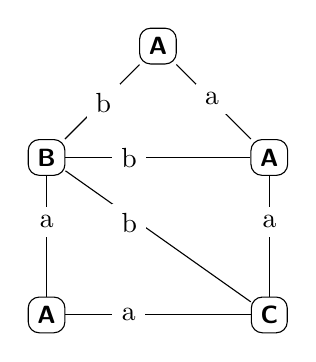
\begin{tikzpicture}[node distance=2cm,node/.style={rounded corners,draw,font=\sffamily\small\bfseries}]
	\node[node] (1) {A};
	\node[node] (2)[below left of=1] {B};
		\node[node] (3)[below right of=1] {A};
		\node[node] (4)[below  of=2] {A};
			\node[node] (5)[below of=3] {C};
	\path
	(1) edge node [minimum width = 1em, fill = white,pos=.25,below left] {b} (2)
		edge node [minimum width = 1em, fill = white,pos=.25,below right]{a} (3)	
	(2) edge node [minimum width = 1em, fill = white,pos=.25,right]{b} (3)
		edge node [minimum width = 1em, fill = white,pos=.25,below]{a} (4)
		edge node [minimum width = 1em, fill = white,pos=.25,below right]{b} (5)
	(3) edge node [minimum width = 1em, fill = white,pos=.25,below]{a} (5)	
	(4) edge node [minimum width = 1em, fill = white,pos=.25,right]{a} (5);	
							
\end{tikzpicture}
\\\textbf{Step 1}
\end{minipage}
 \begin{minipage}{.3\textwidth}
	 \centering
	 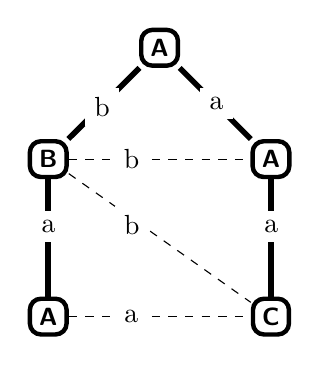
\begin{tikzpicture}[node distance=2cm,node/.style={rounded corners,draw,font=\sffamily\small\bfseries}]
	\node[node,line width=1.6pt] (1) {A};
	\node[node,line width=1.6pt] (2)[below left of=1] {B};
		\node[node,line width=1.6pt] (3)[below right of=1] {A};
		\node[node,line width=1.6pt] (4)[below  of=2] {A};
			\node[node,line width=1.6pt] (5)[below of=3] {C};
	\path
	(1) edge[line width=.7mm] node [minimum width = 1em, fill = white,pos=.25,below left] {b} (2)
		edge[line width=.7mm] node [minimum width = 1em, fill = white,pos=.25,below right]{a} (3)	
	(2) edge[dashed] node [minimum width = 1em, fill = white,pos=.25,right]{b} (3)
		edge[line width=.7mm] node [minimum width = 1em, fill = white,pos=.25,below]{a} (4)
		edge[dashed] node [minimum width = 1em, fill = white,pos=.25,below right]{b} (5)
	(3) edge[line width=.7mm] node [minimum width = 1em, fill = white,pos=.25,below]{a} (5)	
	(4) edge[dashed] node [minimum width = 1em, fill = white,pos=.25,right]{a} (5);	
							
\end{tikzpicture}
\\\textbf{Step 2}
\end{minipage}
\begin{minipage}{.3\textwidth}
	 \centering
	 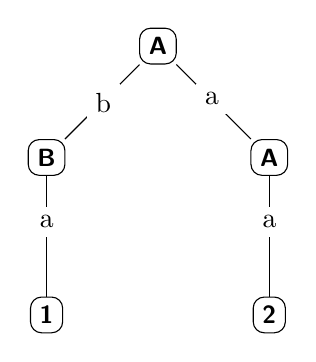
\begin{tikzpicture}[node distance=2cm,node/.style={rounded corners,draw,font=\sffamily\small\bfseries}]
	\node[node] (1) {A};
	\node[node] (2)[below left of=1] {B};
		\node[node] (3)[below right of=1] {A};
		\node[node] (4)[below  of=2] {1};
			\node[node] (5)[below of=3] {2};
	\path
	(1) edge[] node [minimum width = 1em, fill = white,pos=.25,below left] {b} (2)
		edge[] node [minimum width = 1em, fill = white,pos=.25,below right]{a} (3)	
	(2) edge[] node [minimum width = 1em, fill = white,pos=.25,below]{a} (4)
	(3) edge[] node [minimum width = 1em, fill = white,pos=.25,below]{a} (5);							
\end{tikzpicture}
\\\textbf{Step 3}
\end{minipage}
\end{figure}
\end{frame}

\begin{frame}{TurboIso}{Neighbourhood Equivalence Class}
\begin{figure}[h!]
\begin{minipage}{.3\textwidth}
	 \centering
	 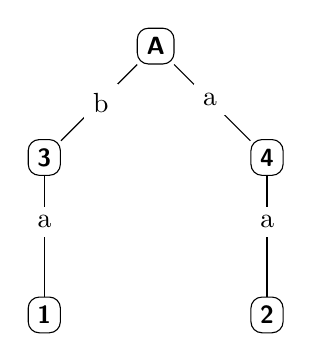
\begin{tikzpicture}[node distance=2cm,node/.style={rounded corners,draw,font=\sffamily\small\bfseries}]
	\node[node] (1) {A};
	\node[node] (2)[below left of=1] {3};
		\node[node] (3)[below right of=1] {4};
		\node[node] (4)[below  of=2] {1};
			\node[node] (5)[below of=3] {2};
	\path
	(1) edge[] node [minimum width = 1em, fill = white,pos=.25,below left] {b} (2)
		edge[] node [minimum width = 1em, fill = white,pos=.25,below right]{a} (3)	
	(2) edge[] node [minimum width = 1em, fill = white,pos=.25,below]{a} (4)
	(3) edge[] node [minimum width = 1em, fill = white,pos=.25,below]{a} (5);							
\end{tikzpicture}
\\\textbf{Step 4}
\end{minipage}
\begin{minipage}{.3\textwidth}
	 \centering
	 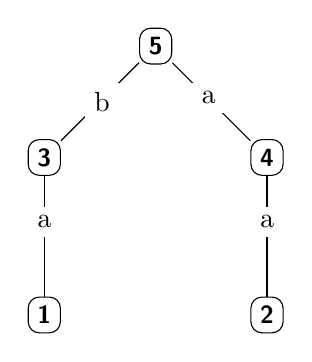
\begin{tikzpicture}[node distance=2cm,node/.style={rounded corners,draw,font=\sffamily\small\bfseries}]
	\node[node] (1) {5};
	\node[node] (2)[below left of=1] {3};
		\node[node] (3)[below right of=1] {4};
		\node[node] (4)[below  of=2] {1};
			\node[node] (5)[below of=3] {2};
	\path
	(1) edge[] node [minimum width = 1em, fill = white,pos=.25,below left] {b} (2)
		edge[] node [minimum width = 1em, fill = white,pos=.25,below right]{a} (3)	
	(2) edge[] node [minimum width = 1em, fill = white,pos=.25,below]{a} (4)
	(3) edge[] node [minimum width = 1em, fill = white,pos=.25,below]{a} (5);							
\end{tikzpicture}
\\\textbf{Step 5}
\end{minipage}
\begin{minipage}{.3\textwidth}
	 \centering
	 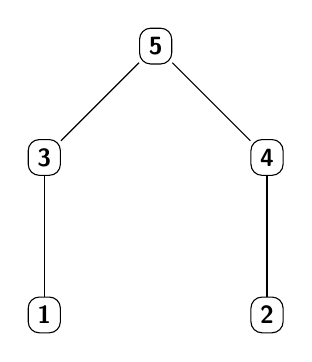
\begin{tikzpicture}[node distance=2cm,node/.style={rounded corners,draw,font=\sffamily\small\bfseries}]
	\node[node] (1) {5};
	\node[node] (2)[below left of=1] {3};
		\node[node] (3)[below right of=1] {4};
		\node[node] (4)[below  of=2] {1};
			\node[node] (5)[below of=3] {2};
	\path
	(1) edge[] node [] {} (2)
		edge[] node []{} (3)	
	(2) edge[] node []{} (4)
	(3) edge[] node []{} (5);							
\end{tikzpicture}
\\\textbf{Step 6}
\end{minipage}
\end{figure}
\end{frame}

\begin{frame}{TurboIso}{Neighbourhood Equivalence Class}
\begin{figure}[h!]
\begin{minipage}{.3\textwidth}
\centering
\hfill \\

\begin{tikzpicture}[node distance=2cm,node/.style={rounded corners,draw,font=\sffamily\small\bfseries}]
\node[node,label=NEC 1] (2){A};
\end{tikzpicture}\\
\hfill \\

\begin{tikzpicture}[node distance=2cm,node/.style={rounded corners,draw,font=\sffamily\small\bfseries}]
\node[node,label=NEC 2] (2){C};
\end{tikzpicture}\\
\hfill \\
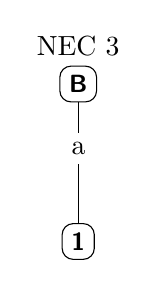
\begin{tikzpicture}[node distance=2cm,node/.style={rounded corners,draw,font=\sffamily\small\bfseries}]

\node[node,label=NEC 3] (2){B};
\node[node] (3)[below of=2]{1};
\path
	(2)	 edge node[minimum width = 1em, fill = white,pos=.25,below ] {a} (3);
\end{tikzpicture}
\end{minipage}
\begin{minipage}{.3\textwidth}
\centering
\hfill \\
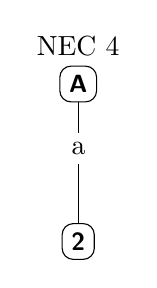
\begin{tikzpicture}[node distance=2cm,node/.style={rounded corners,draw,font=\sffamily\small\bfseries}]

\node[node,label=NEC 4] (2){A};
\node[node] (3)[below of=2]{2};
\path
	(2)	 edge node[minimum width = 1em, fill = white,pos=.25,below ] {a} (3);
\end{tikzpicture}
\hfill \\
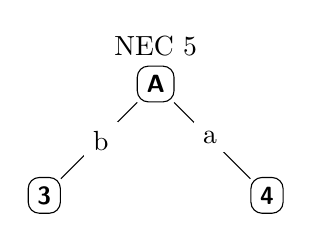
\begin{tikzpicture}[node distance=2cm,node/.style={rounded corners,draw,font=\sffamily\small\bfseries}]

\node[node,label=NEC 5] (2){A};
\node[node] (3)[below left of=2]{3};
\node[node] (4)[below right of=2]{4};
\path
	(2)	 edge node[minimum width = 1em, fill = white,pos=.25,below left] {b} (3)
		 edge node[minimum width = 1em, fill = white,pos=.25,below right] {a} (4);
\end{tikzpicture}
\\Classes
\end{minipage}
\end{figure}
%  \begin{figure}[h]
% \centering
%%\centering
%\begin{tikzpicture}[node distance=2cm]
%\node[circle,draw] (1)[]{5};
%\node[circle,draw] (3)[below of=1]{4};
%\node[circle,draw] (2)[left of=3]{2};
%
%\node[circle,draw] (4)[ right of=3]{3};
%\node[circle,draw] (5)[below of=2]{1};
%\node[circle,draw] (6)[left of=5]{1};
%\node[circle,draw] (7)[below of=3]{2};
%\node[circle,draw] (8)[right of=7]{1};
%\node[circle,draw] (9)[right of=8]{1};
%\node[circle,draw] (10)[below left of=7]{1};
%\node[circle,draw] (11)[below right of=7]{1};
%\path
%	(1) edge node{} (2)
%		 edge node{} (3)
%		 edge node{} (4)
%	(2) edge node{} (5)
%		edge node{} (6)
%	(3) edge node{} (7)
%		edge node{} (8)
%	(4) edge node{} (9)
%	(7) edge node{} (10)
%		edge node{} (11);	
%\end{tikzpicture}
%
% \caption{NEC Numbering}
%\end{figure}
\end{frame}
\begin{frame}
\begin{block}{Parallel NEC}
    \begin{itemize}
    \item Identify neighbourhood
    \begin{enumerate}
        \item(Parallel) If all neighbours have numbered
        \item Find the hash of neighbourhood
    \end{enumerate}
    \item Use thrust-Scan to assign unique numbers
    \item Find unique number for the neighbourhood
    \begin{enumerate}
        \item(Parallel) find the hash of neighbourhood
        \item Assign the unique number at the hash location
    \end{enumerate}
    \end{itemize}
\end{block}
\end{frame}
\begin{frame}{CVS Generation}
\begin{figure}[h!]
\begin{minipage}{.4\textwidth}
	\centering
	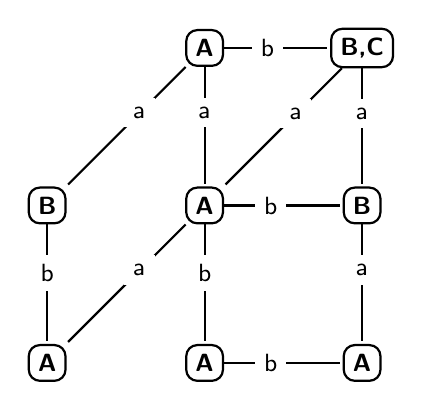
\begin{tikzpicture}[shorten >=1pt,auto,node distance=2cm,
                    thick,main node/.style={rounded corners,draw,font=\sffamily\small\bfseries}]

  \node[main node] (1) {A};
  \node[main node] (2) [right of=1] {B,C}; 
  \node[main node] (4) [below of =1] {A};
  \node[main node] (3) [left of=4] {B};
     \node[main node] (5) [below of=2] {B};
    \node[main node] (6) [below of=3] {A};
    \node[main node] (7) [below of=4] {A};
\node[main node] (8) [below of=5] {A};
  \path[every node/.style={font=\sffamily\small}]
    (1) edge[] node [minimum width = 1em, fill = white,pos=.25,right] {b} (2)
        edge[] node[minimum width = 1em, fill = white,pos=.25,below left] {a} (3)
        edge[] node[minimum width = 1em, fill = white,pos=.25,below] {a} (4)
    (2) edge[] node [minimum width = 1em, fill = white,pos=.25,below left] {a} (4)
        edge node [minimum width = 1em, fill = white,pos=.25,below] {a} (5)
    (3) edge[] node [minimum width = 1em, fill = white,pos=.25,below] {b} (6)
    (4) edge node [minimum width = 1em, fill = white,pos=.25,below] {b} (7)
    	edge[] node [minimum width = 1em, fill = white,pos=.25,below left] {a} (6) 
    	edge node [minimum width = 1em, fill = white,pos=.25,right] {b} (5) 
    (5) edge node [minimum width = 1em, fill = white,pos=.25,below] {a} (8)
    (7) edge node [minimum width = 1em, fill = white,pos=.25,right] {b} (8);	   
\end{tikzpicture}
\\\textbf{Step 1}
\end{minipage}
\begin{minipage}{.4\textwidth}
	\centering
	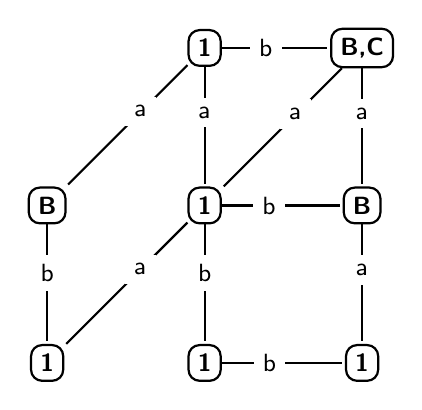
\begin{tikzpicture}[shorten >=1pt,auto,node distance=2cm,
                    thick,main node/.style={rounded corners,draw,font=\sffamily\small\bfseries}]

  \node[main node] (1) {1};
  \node[main node] (2) [right of=1] {B,C}; 
  \node[main node] (4) [below of =1] {1};
  \node[main node] (3) [left of=4] {B};
     \node[main node] (5) [below of=2] {B};
    \node[main node] (6) [below of=3] {1};
    \node[main node] (7) [below of=4] {1};
\node[main node] (8) [below of=5] {1};
  \path[every node/.style={font=\sffamily\small}]
    (1) edge[] node [minimum width = 1em, fill = white,pos=.25,right] {b} (2)
        edge[] node[minimum width = 1em, fill = white,pos=.25,below left] {a} (3)
        edge[] node[minimum width = 1em, fill = white,pos=.25,below] {a} (4)
    (2) edge[] node [minimum width = 1em, fill = white,pos=.25,below left] {a} (4)
        edge node [minimum width = 1em, fill = white,pos=.25,below] {a} (5)
    (3) edge[] node [minimum width = 1em, fill = white,pos=.25,below] {b} (6)
    (4) edge node [minimum width = 1em, fill = white,pos=.25,below] {b} (7)
    	edge[] node [minimum width = 1em, fill = white,pos=.25,below left] {a} (6) 
    	edge node [minimum width = 1em, fill = white,pos=.25,right] {b} (5) 
    (5) edge node [minimum width = 1em, fill = white,pos=.25,below] {a} (8)
    (7) edge node [minimum width = 1em, fill = white,pos=.25,right] {b} (8);	   
\end{tikzpicture}
\\\textbf{Step 2}
\end{minipage}
\end{figure}
\end{frame}
\begin{frame}{CVS Generation}
\begin{figure}[h!]
\begin{minipage}{.4\textwidth}
	\centering
	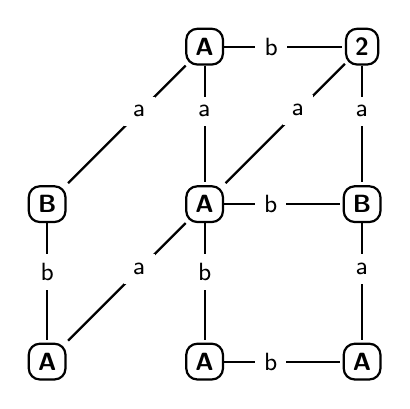
\begin{tikzpicture}[shorten >=1pt,auto,node distance=2cm,
                    thick,main node/.style={rounded corners,draw,font=\sffamily\small\bfseries}]

  \node[main node] (1) {A};
  \node[main node] (2) [right of=1] {2}; 
  \node[main node] (4) [below of =1] {A};
  \node[main node] (3) [left of=4] {B};
     \node[main node] (5) [below of=2] {B};
    \node[main node] (6) [below of=3] {A};
    \node[main node] (7) [below of=4] {A};
\node[main node] (8) [below of=5] {A};
  \path[every node/.style={font=\sffamily\small}]
    (1) edge[] node [minimum width = 1em, fill = white,pos=.25,right] {b} (2)
        edge[] node[minimum width = 1em, fill = white,pos=.25,below left] {a} (3)
        edge[] node[minimum width = 1em, fill = white,pos=.25,below] {a} (4)
    (2) edge[] node [minimum width = 1em, fill = white,pos=.25,below left] {a} (4)
        edge node [minimum width = 1em, fill = white,pos=.25,below] {a} (5)
    (3) edge[] node [minimum width = 1em, fill = white,pos=.25,below] {b} (6)
    (4) edge node [minimum width = 1em, fill = white,pos=.25,below] {b} (7)
    	edge[] node [minimum width = 1em, fill = white,pos=.25,below left] {a} (6) 
    	edge node [minimum width = 1em, fill = white,pos=.25,right] {b} (5) 
    (5) edge node [minimum width = 1em, fill = white,pos=.25,below] {a} (8)
    (7) edge node [minimum width = 1em, fill = white,pos=.25,right] {b} (8);	   
\end{tikzpicture}
\\\textbf{Step 3}
\end{minipage}
\begin{minipage}{.4\textwidth}
	\centering
	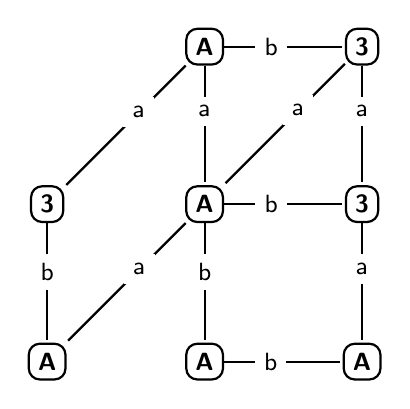
\begin{tikzpicture}[shorten >=1pt,auto,node distance=2cm,
                    thick,main node/.style={rounded corners,draw,font=\sffamily\small\bfseries}]

  \node[main node] (1) {A};
  \node[main node] (2) [right of=1] {3}; 
  \node[main node] (4) [below of =1] {A};
  \node[main node] (3) [left of=4] {3};
     \node[main node] (5) [below of=2] {3};
    \node[main node] (6) [below of=3] {A};
    \node[main node] (7) [below of=4] {A};
\node[main node] (8) [below of=5] {A};
  \path[every node/.style={font=\sffamily\small}]
    (1) edge[] node [minimum width = 1em, fill = white,pos=.25,right] {b} (2)
        edge[] node[minimum width = 1em, fill = white,pos=.25,below left] {a} (3)
        edge[] node[minimum width = 1em, fill = white,pos=.25,below] {a} (4)
    (2) edge[] node [minimum width = 1em, fill = white,pos=.25,below left] {a} (4)
        edge node [minimum width = 1em, fill = white,pos=.25,below] {a} (5)
    (3) edge[] node [minimum width = 1em, fill = white,pos=.25,below] {b} (6)
    (4) edge node [minimum width = 1em, fill = white,pos=.25,below] {b} (7)
    	edge[] node [minimum width = 1em, fill = white,pos=.25,below left] {a} (6) 
    	edge node [minimum width = 1em, fill = white,pos=.25,right] {b} (5) 
    (5) edge node [minimum width = 1em, fill = white,pos=.25,below] {a} (8)
    (7) edge node [minimum width = 1em, fill = white,pos=.25,right] {b} (8);	   
\end{tikzpicture}
\\\textbf{Step 4}
\end{minipage}
\end{figure}
\end{frame}
\begin{frame}{CVS Generation}
\begin{figure}[h!]
\begin{minipage}{.4\textwidth}
	\centering
	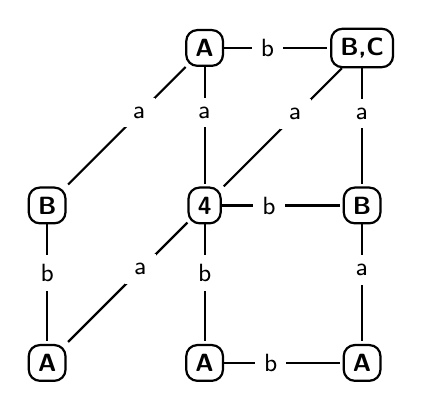
\begin{tikzpicture}[shorten >=1pt,auto,node distance=2cm,
                    thick,main node/.style={rounded corners,draw,font=\sffamily\small\bfseries}]

  \node[main node] (1) {A};
  \node[main node] (2) [right of=1] {B,C}; 
  \node[main node] (4) [below of =1] {4};
  \node[main node] (3) [left of=4] {B};
     \node[main node] (5) [below of=2] {B};
    \node[main node] (6) [below of=3] {A};
    \node[main node] (7) [below of=4] {A};
\node[main node] (8) [below of=5] {A};
  \path[every node/.style={font=\sffamily\small}]
    (1) edge[] node [minimum width = 1em, fill = white,pos=.25,right] {b} (2)
        edge[] node[minimum width = 1em, fill = white,pos=.25,below left] {a} (3)
        edge[] node[minimum width = 1em, fill = white,pos=.25,below] {a} (4)
    (2) edge[] node [minimum width = 1em, fill = white,pos=.25,below left] {a} (4)
        edge node [minimum width = 1em, fill = white,pos=.25,below] {a} (5)
    (3) edge[] node [minimum width = 1em, fill = white,pos=.25,below] {b} (6)
    (4) edge node [minimum width = 1em, fill = white,pos=.25,below] {b} (7)
    	edge[] node [minimum width = 1em, fill = white,pos=.25,below left] {a} (6) 
    	edge node [minimum width = 1em, fill = white,pos=.25,right] {b} (5) 
    (5) edge node [minimum width = 1em, fill = white,pos=.25,below] {a} (8)
    (7) edge node [minimum width = 1em, fill = white,pos=.25,right] {b} (8);	   
\end{tikzpicture}
\\\textbf{Step 5}
\end{minipage}
\begin{minipage}{.4\textwidth}
	\centering
	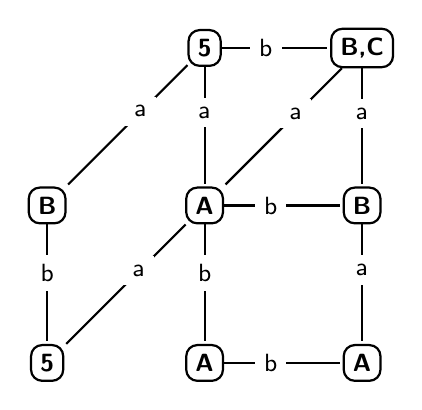
\begin{tikzpicture}[shorten >=1pt,auto,node distance=2cm,
                    thick,main node/.style={rounded corners,draw,font=\sffamily\small\bfseries}]

  \node[main node] (1) {5};
  \node[main node] (2) [right of=1] {B,C}; 
  \node[main node] (4) [below of =1] {A};
  \node[main node] (3) [left of=4] {B};
     \node[main node] (5) [below of=2] {B};
    \node[main node] (6) [below of=3] {5};
    \node[main node] (7) [below of=4] {A};
\node[main node] (8) [below of=5] {A};
  \path[every node/.style={font=\sffamily\small}]
    (1) edge[] node [minimum width = 1em, fill = white,pos=.25,right] {b} (2)
        edge[] node[minimum width = 1em, fill = white,pos=.25,below left] {a} (3)
        edge[] node[minimum width = 1em, fill = white,pos=.25,below] {a} (4)
    (2) edge[] node [minimum width = 1em, fill = white,pos=.25,below left] {a} (4)
        edge node [minimum width = 1em, fill = white,pos=.25,below] {a} (5)
    (3) edge[] node [minimum width = 1em, fill = white,pos=.25,below] {b} (6)
    (4) edge node [minimum width = 1em, fill = white,pos=.25,below] {b} (7)
    	edge[] node [minimum width = 1em, fill = white,pos=.25,below left] {a} (6) 
    	edge node [minimum width = 1em, fill = white,pos=.25,right] {b} (5) 
    (5) edge node [minimum width = 1em, fill = white,pos=.25,below] {a} (8)
    (7) edge node [minimum width = 1em, fill = white,pos=.25,right] {b} (8);	   
\end{tikzpicture}
\\\textbf{Step 6}
\end{minipage}
\end{figure}
\end{frame}
\begin{frame}{CVS Generation}
\begin{figure}[h!]
\begin{minipage}{.4\textwidth}
	\centering
	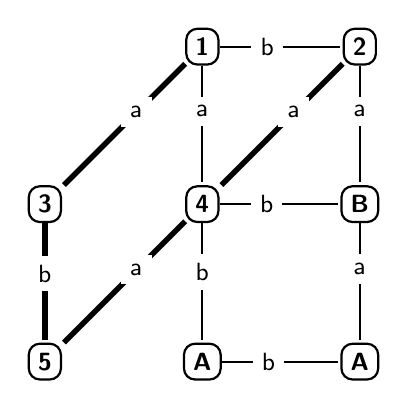
\begin{tikzpicture}[shorten >=1pt,auto,node distance=2cm,
                    thick,main node/.style={rounded corners,draw,font=\sffamily\small\bfseries}]

  \node[main node] (1) {1};
  \node[main node] (2) [right of=1] {2}; 
  \node[main node] (4) [below of =1] {4};
  \node[main node] (3) [left of=4] {3};
     \node[main node] (5) [below of=2] {B};
    \node[main node] (6) [below of=3] {5};
    \node[main node] (7) [below of=4] {A};
\node[main node] (8) [below of=5] {A};
  \path[every node/.style={font=\sffamily\small}]
    (1) edge[] node [minimum width = 1em, fill = white,pos=.25,right] {b} (2)
        edge[line width=.7mm] node[minimum width = 1em, fill = white,pos=.25,below left] {a} (3)
        edge[] node[minimum width = 1em, fill = white,pos=.25,below] {a} (4)
    (2) edge[line width=.7mm] node [minimum width = 1em, fill = white,pos=.25,below left] {a} (4)
        edge node [minimum width = 1em, fill = white,pos=.25,below] {a} (5)
    (3) edge[line width=.7mm] node [minimum width = 1em, fill = white,pos=.25,below] {b} (6)
    (4) edge node [minimum width = 1em, fill = white,pos=.25,below] {b} (7)
    	edge[line width=.7mm] node [minimum width = 1em, fill = white,pos=.25,below left] {a} (6) 
    	edge node [minimum width = 1em, fill = white,pos=.25,right] {b} (5) 
    (5) edge node [minimum width = 1em, fill = white,pos=.25,below] {a} (8)
    (7) edge node [minimum width = 1em, fill = white,pos=.25,right] {b} (8);	   
\end{tikzpicture}
\\\textbf{Step 7}
\end{minipage}
\begin{minipage}{.4\textwidth}
	\centering
	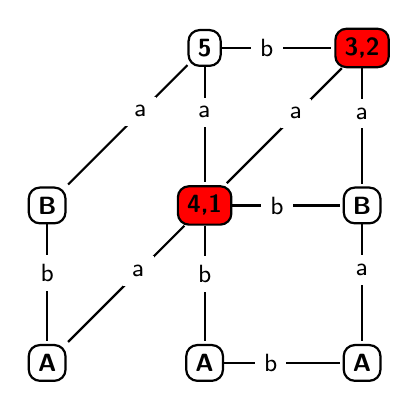
\begin{tikzpicture}[shorten >=1pt,auto,node distance=2cm,
                    thick,main node/.style={rounded corners,draw,font=\sffamily\small\bfseries}]

  \node[main node] (1) {5};
  \node[main node,fill={rgb:red,4;green,0;yellow,0}] (2) [right of=1] {3,2}; 
  \node[main node,fill={rgb:red,4;green,0;yellow,0}] (4) [below of =1] {4,1};
  \node[main node] (3) [left of=4] {B};
     \node[main node] (5) [below of=2] {B};
    \node[main node] (6) [below of=3] {A};
    \node[main node] (7) [below of=4] {A};
\node[main node] (8) [below of=5] {A};
  \path[every node/.style={font=\sffamily\small}]
    (1) edge[] node [minimum width = 1em, fill = white,pos=.25,right] {b} (2)
        edge[] node[minimum width = 1em, fill = white,pos=.25,below left] {a} (3)
        edge[] node[minimum width = 1em, fill = white,pos=.25,below] {a} (4)
    (2) edge[] node [minimum width = 1em, fill = white,pos=.25,below left] {a} (4)
        edge node [minimum width = 1em, fill = white,pos=.25,below] {a} (5)
    (3) edge[] node [minimum width = 1em, fill = white,pos=.25,below] {b} (6)
    (4) edge node [minimum width = 1em, fill = white,pos=.25,below] {b} (7)
    	edge[] node [minimum width = 1em, fill = white,pos=.25,below left] {a} (6) 
    	edge node [minimum width = 1em, fill = white,pos=.25,right] {b} (5) 
    (5) edge node [minimum width = 1em, fill = white,pos=.25,below] {a} (8)
    (7) edge node [minimum width = 1em, fill = white,pos=.25,right] {b} (8);	   
\end{tikzpicture}
\\\textbf{Step 8}
\end{minipage}
\end{figure}
\end{frame}

%\begin{block}{Parallel Candidate Set Generation}
%
%    \begin{itemize}
%    \item Foreach NECs
%    \item (Parallel) Check for existence of the neighbourhood 
%    \end{itemize}
%    \end{block}
%     \begin{figure}[h]
% \centering
%%\centering
%\begin{tikzpicture}[node distance=2cm]
%\node[circle,draw,label={1,2,3,4,5}] (1)[]{};
%\node[circle,draw,label={1,2,3,4}] (3)[below of=1]{};
%\node[circle,draw,label={1,2,3,4}] (2)[left of=3]{};
%
%\node[circle,draw,label={1,2,3,4}] (4)[ right of=3]{};
%\node[circle,draw,label={1,3}] (5)[below of=2]{};
%\node[circle,draw,label={1,3}] (6)[left of=5]{};
%\node[circle,draw,label={1,2,3,4}] (7)[below of=3]{};
%\node[circle,draw,label={1,3}] (8)[right of=7]{};
%\node[circle,draw,label={1,3}] (9)[right of=8]{};
%\node[circle,draw,label={1,3}] (10)[below left of=7]{};
%\node[circle,draw,label={1,3}] (11)[below right of=7]{};
%\path
%	(1) edge node{} (2)
%		 edge node{} (3)
%		 edge node{} (4)
%	(2) edge node{} (5)
%		edge node{} (6)
%	(3) edge node{} (7)
%		edge node{} (8)
%	(4) edge node{} (9)
%	(7) edge node{} (10)
%		edge node{} (11);	
%\end{tikzpicture}
%\end{figure}

%\begin{frame}{Failure}
%\begin{block}{Using primes}
%    \begin{itemize}
%    \item A prime is assigned for each unique pattern
%    \item A composite is given if the prime factor subgraphs are present in that node.
%    \item Because of the propagation of primes every node was getting every prime id making the algorithm ineffective.
%    \end{itemize}
%
%\end{block}
%\end{frame}
%\begin{frame}
%    \begin{figure}[h]
% \centering
%%\centering
%\begin{minipage}{.6\textwidth}
%\begin{tikzpicture}[node distance=2cm]
%\node[circle,draw,label=v1] (1)[]{315};
%\node[circle,draw,label=v2] (3)[below of=1]{10};
%\node[circle,draw,label=v3] (2)[left of=3]{4};
%\node[circle,draw,label=v4] (4)[ right of=3]{2};
%\node[circle,draw,label=v5] (5)[below of=2]{1};
%\node[circle,draw,label=v6] (6)[left of=5]{1};
%\node[circle,draw,label=v7] (7)[below of=3]{4};
%\node[circle,draw,label=v8] (8)[right of=7]{1};
%\node[circle,draw,label=v9] (9)[right of=8]{1};
%\node[circle,draw,label=v10] (10)[below left of=7]{1};
%\node[circle,draw,label=v11] (11)[below right of=7]{1};
%\path
%	(1) edge node{} (2)
%		 edge node{} (3)
%		 edge node{} (4)
%	(2) edge node{} (5)
%		edge node{} (6)
%	(3) edge node{} (7)
%		edge node{} (8)
%	(4) edge node{} (9)
%	(7) edge node{} (10)
%		edge node{} (11);	
%\end{tikzpicture}
%\end{minipage}
%\begin{minipage}{.3\textwidth}
%\centering
%\begin{tikzpicture}[scale=0.1,every node/.style={scale=0.6}]
%\node[circle,draw] (5)[]{7};
%\node[circle,draw] (1)[below of=5]{5};
%\node[circle,draw] (2)[below of=1]{4};
%\node[circle,draw] (3)[below left of=2]{1};
%\node[circle,draw] (4)[below right of=2]{1};
%\path
%	(5) edge node{} (1)
%	(1) edge node{} (2)
%	(2)	 edge node{} (3)
%		 edge node{} (4);
%\end{tikzpicture}\\Intermediate graph \hfill \\
%\begin{tikzpicture}[scale=0.1,every node/.style={scale=0.6}]
%
%\node[circle,draw] (1)[]{3};
%\node[circle,draw] (2)[below of=1]{2};
%\node[circle,draw] (3)[below of=2]{1};
%\path
%	(5) edge node{} (1)
%	(1) edge node{} (2)
%	(2)	 edge node{} (3);
%\end{tikzpicture}
%\\Intermediate Graph
%\end{minipage}
% \caption{NEC based on primes}
%\end{figure}
%\end{frame}
% \begin{frame}{Label sparse coding Algorithm}
% \end{frame}

% \begin{frame}{Dimensionality Reduction}{Multi-label Linear Embedding (MLE)}
% Learn a transformation matrix $P \in \mathbb{R}^{m_1 \times m_2}$ ($m_2 < m_1$).
% \begin{itemize}

% \item {Using $W^1$} :
%   The samples having the label sets should be very near or similar to each other in the transformed space.
%   \begin{equation}\label{w1}
%   \frac{1}{2}\underset{ij}\sum \left \| P^T\mathbf{x}_i - P^T\mathbf{x}_j \right \|^2W_{ij}^1, \hspace{0.2cm} s.t \hspace{0.2cm}P^TP = I
%   \end{equation}

 
% \item Semantic similarities between image and the rest of images should be retained in the new space. 

% \begin{equation}\label{w2}
%   \underset{P}min\frac{1}{2}\underset{i}\sum \left \| P^T\mathbf{x}_i -\underset{j}\sum W^2_{ij} P^T\mathbf{x}_j \right \|^2, \hspace{0.2cm} s.t \hspace{0.2cm}P^TP = I
%   \end{equation}
%   \item Combining above two objective functions $P$ can be found by 
%   \begin{equation}
% \underset{P}min  \hspace{0.2cm} Tr(P^TXMX^TP)
% \end{equation}
% \end{itemize}
%  \begin{figure}
%     \centering
%     \includegraphics[width=0.3\textwidth, height = 2cm]{PartialLabel.jpg}
%   % \caption {Broad Category - Beach  \pause \color{red} Sand, mountain, sky, clouds}
   
%     \label{fig:my_label}
% \end{figure}

% \end{frame}

\begin{frame}{Experiments - Data Graph Size varies}
\begin{figure}[h]
 \centering
\includegraphics[width=.5\textwidth]{Dchange.png}

 \label{fig:dchange}
\end{figure}
\begin{block}{Inferences}
    \begin{itemize}
    \item Density of data graph is crucial
%    \item The Data and Query graphs are cliques.
%    \item The code is run on a NVIDIA GPU (580Mhz) with CUDA 7.5 support
    \end{itemize}
\end{block}
\end{frame}
\begin{frame}{Experiments - Query Graph Size varies}
\begin{figure}[h]
 \centering
\includegraphics[width=.5\textwidth]{Qchange.png}

 \label{fig:dchange}
\end{figure}
\begin{block}{Inferences}
    \begin{itemize}
    \item Query graph size affects stage 2
%    \item The Data and Query graphs are cliques.
%    \item The code is run on a NVIDIA GPU (580Mhz) with CUDA 7.5 support
    \end{itemize}
\end{block}
\end{frame}
\begin{frame}{Experiments - Facebook Data}
\begin{figure}[h]
 \centering
\includegraphics[width=.5\textwidth]{fb.png}

 \label{fig:dchange}
\end{figure}
\begin{block}{Inferences}
    \begin{itemize}
    \item 4039 nodes and 88234 edges.Highly Dense.
%    \item The Data and Query graphs are cliques.
%    \item The code is run on a NVIDIA GPU (580Mhz) with CUDA 7.5 support
    \end{itemize}
\end{block}
\end{frame}

\begin{frame}{Experiments - Condense Matter collaboration network Dataset}
\begin{figure}[h]
 \centering
\includegraphics[width=.5\textwidth]{CA.png}

 \label{fig:dchange}
\end{figure}
\begin{block}{Inferences}
    \begin{itemize}
    \item 23133 nodes and 93497 edges.
%    \item The Data and Query graphs are cliques.
%    \item The code is run on a NVIDIA GPU (580Mhz) with CUDA 7.5 support
    \end{itemize}
\end{block}
\end{frame}
%\begin{table}[htbp]
%    \centering
%\caption{Time to Execute(in s)}
%    \label{tab:mytable}
%\begin{tabular}{|l|l|l|}
%    \specialrule{1pt}{1pt}{1pt}
%\diaghead{Scoreexp}{Query}{Data}   & 10     & 100  \\
%    \hline%\addlinespace
%    3     & 2.8     & 3      \\ \hline
%    5     & 3.6   & 3*      \\ \hline
%    10     & 4.8     & 60*     \\ \hline
%    
%   % \bottomrule
%\end{tabular}%
%  \label{tab:addlabel}%
%\end{table}



\begin{frame}
\frametitle{Dynamic Queries}
\begin{block}{Intermediate Results}
\end{block}
\begin{figure}[h]
 \centering
%\centering
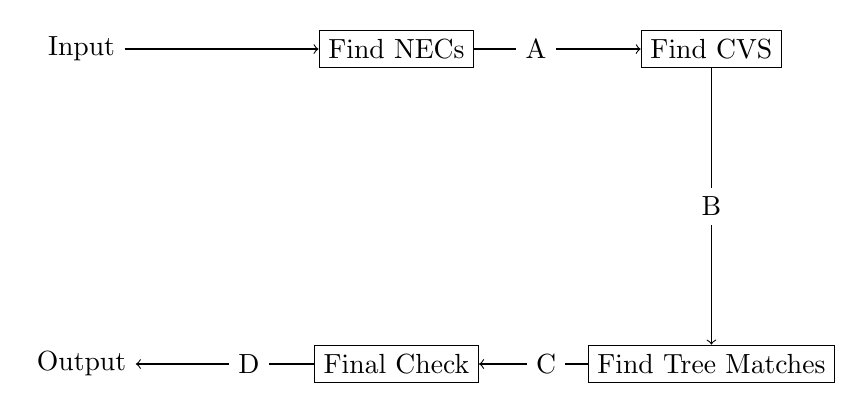
\begin{tikzpicture}[node distance=4cm]
\node[draw=none](6)[]{Input};
\node[rectangle,draw] (1)[right of=6]{Find NECs};
\node[rectangle,draw] (2)[right of=1]{Find CVS};
\node[rectangle,draw] (3)[below of=2]{Find Tree Matches};
\node[rectangle,draw] (4)[left of=3]{Final Check};
\node[draw=none](5)[left of =4]{Output};
\path[->]
	(6) edge node{} (1)
	(1) edge node[minimum width = 1em, fill = white,pos=.25,right] {A} (2)
	(2) edge node[minimum width = 1em, fill = white,pos=.5]{B} (3)
	(3) edge node[minimum width = 1em, fill = white,pos=.2,left]{C} (4)
	(4) edge node[minimum width = 1em, fill = white,pos=.25,left] {D} (5);
\end{tikzpicture}
\end{figure}
\end{frame}
\begin{frame}
\frametitle{Queries }
\begin{table}[H]
\centering
\begin{tabular}{|m{3cm}|m{3cm}|m{3cm}|m{3cm}|}
\hline
\textbf{}                                  & \textbf{Query Add Edge}                     & \textbf{Query Remove edge}                                 & \textbf{Query Unchanged} \\ \hline
\textbf{Data Add Edge}                                  & \textbf{Dificult}                     & \textbf{Difficult}                                 & \textbf{Easy} \\ \hline
\textbf{Data Remove Edge}                                  & \textbf{Easy}                     & \textbf{Difficult}                                 & \textbf{Easy} \\ \hline
\textbf{Data Unchanged}                                  & \textbf{Easy}                     & \textbf{Difficult}                                 & \textbf{Static} \\ \hline
\end{tabular}
%\label{tab:lit}
\end{table}
\end{frame}
\begin{frame}
\frametitle{Trivial Cases }
\begin{block}{Adding Edge to Query Graph}
\begin{enumerate}
\item need to check only the previous answers 
\end{enumerate}

\end{block}
\begin{block}{Deleting Edge from Data Graph}
\begin{enumerate}
\item need to check only the previous answers 
\end{enumerate}

\end{block}
\end{frame}
\begin{frame}
\frametitle{Delete Edge in Query Graph}
\begin{figure}[h]
 \centering
	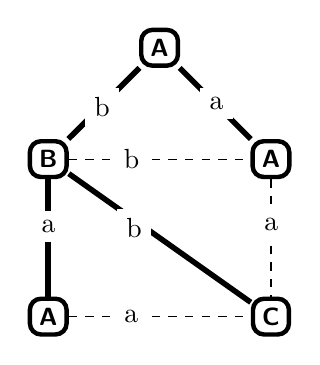
\begin{tikzpicture}[node distance=2cm,node/.style={rounded corners,draw,font=\sffamily\small\bfseries}]
	\node[node,line width=1.6pt] (1) {A};
	\node[node,line width=1.6pt] (2)[below left of=1] {B};
		\node[node,line width=1.6pt] (3)[below right of=1] {A};
		\node[node,line width=1.6pt] (4)[below  of=2] {A};
			\node[node,line width=1.6pt] (5)[below of=3] {C};
	\path
	(1) edge[line width=.7mm] node [minimum width = 1em, fill = white,pos=.25,below left] {b} (2)
		edge[line width=.7mm] node [minimum width = 1em, fill = white,pos=.25,below right]{a} (3)	
	(2) edge[dashed] node [minimum width = 1em, fill = white,pos=.25,right]{b} (3)
		edge[line width=.7mm] node [minimum width = 1em, fill = white,pos=.25,below]{a} (4)
		edge[line width=.7mm] node [minimum width = 1em, fill = white,pos=.25,below right]{b} (5)
	(3) edge[dashed] node [minimum width = 1em, fill = white,pos=.25,below]{a} (5)	
	(4) edge[dashed] node [minimum width = 1em, fill = white,pos=.25,right]{a} (5);	
							
\end{tikzpicture}
 \caption{Tree in Query Grpah}
 \label{fig:tree}
\end{figure}

\begin{enumerate}
\item Delete tree edge
\item Delete non-tree edge
\end{enumerate}

\end{frame}

\begin{frame}
\frametitle{Deleting Edge from Query Graph }
\begin{block}{Deleting a non-tree edge}
\begin{enumerate}
\item need to go through all the tree matching(C)
\end{enumerate}

\end{block}
\begin{block}{Deleting a tree edge}
\begin{enumerate}
\item All the nodes in the path from u to root(parent,grand-parent,.. of u) should recalculate the CVS
\end{enumerate}

\end{block}
\end{frame}
\begin{frame}
\frametitle{Algorithm-Deleting a tree edge }
\begin{algorithm}[H]
\caption{Dynamic tree edge deletion of thread t}
\textbf{Input}: Data Graph $D$,Query Graph $Q$,Delete u-v(u is parent of v).\\
\textbf{Output}: CVS updates.\\
\begin{algorithmic}
 \item \begin{enumerate}
 \item w=v
\item for each parent of w(till root)
 \begin{enumerate}
\item mark w for t
\end{enumerate}
\item for each parent of w(till root)
 \begin{enumerate}
\item if mark at w is t, acquire lock for w
\end{enumerate}
\item for each parent of w(till root)
\begin{enumerate}
\item if mark at w is t and able to acquire locks for all child of w 
\item Recompute NEC of w
\item if not a previously computed NEC then
\item  \hspace{10mm}C(w)=$FindCandidates$(w,D) update
\item Release all locks
\end{enumerate}
\end{enumerate}
\end{algorithmic}
\label{alg:treeedge}
\end{algorithm}
\end{frame}

\begin{frame}
\frametitle{Deleting Edge in Query Graph }

\begin{figure}[h!]
 \centering
 \begin{minipage}{.3\textwidth}
	 \centering
	 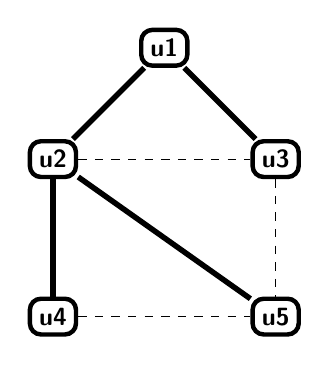
\begin{tikzpicture}[node distance=2cm,node/.style={rounded corners,draw,font=\sffamily\small\bfseries}]
	\node[node,line width=1.6pt] (1) {u1};
	\node[node,line width=1.6pt] (2)[below left of=1] {u2};
		\node[node,line width=1.6pt] (3)[below right of=1] {u3};
		\node[node,line width=1.6pt] (4)[below  of=2] {u4};
			\node[node,line width=1.6pt] (5)[below of=3] {u5};
	\path
	(1) edge[line width=.7mm] node [] {} (2)
		edge[line width=.7mm] node []{} (3)	
	(2) edge[dashed] node []{} (3)
		edge[line width=.7mm] node []{} (4)
		edge[line width=.7mm] node []{} (5)
	(3) edge[dashed] node []{} (5)	
	(4) edge[dashed] node []{} (5);	
							
\end{tikzpicture}
\\\textbf{Step 1}
\end{minipage}
\begin{minipage}{.3\textwidth}
	 \centering
	 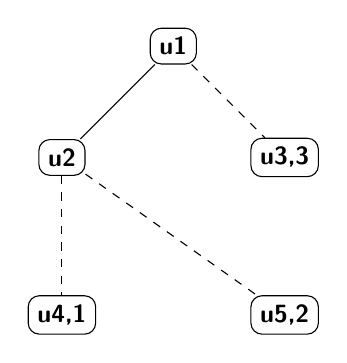
\begin{tikzpicture}[node distance=2cm,node/.style={rounded corners,draw,font=\sffamily\small\bfseries}]
	\node[node] (1) {u1};
	\node[node] (2)[below left of=1] {u2};
		\node[node] (3)[below right of=1] {u3,3};
		\node[node] (4)[below  of=2] {u4,1};
			\node[node] (5)[below of=3] {u5,2};
	\path
	(1) edge[] node [] {} (2)
		edge[dashed] node []{} (3)	
	(2) edge[dashed] node []{} (4)
		edge[dashed] node []{} (5);							
\end{tikzpicture}
\\\textbf{Step 2}
\end{minipage}
\begin{minipage}{.35\textwidth}
	 \centering
	 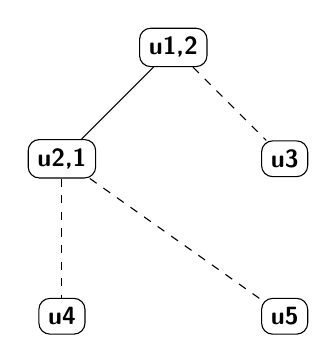
\begin{tikzpicture}[node distance=2cm,node/.style={rounded corners,draw,font=\sffamily\small\bfseries}]
	\node[node] (1) {u1,2};
	\node[node] (2)[below left of=1] {u2,1};
		\node[node] (3)[below right of=1] {u3};
		\node[node] (4)[below  of=2] {u4};
			\node[node] (5)[below of=3] {u5};
	\path
	(1) edge[] node [] {} (2)
		edge[dashed] node []{} (3)	
	(2) edge[dashed] node []{} (4)
		edge[dashed] node []{} (5);							
\end{tikzpicture}
\\\textbf{Step 3}
\end{minipage}
\end{figure}
\end{frame}
\begin{frame}
\frametitle{Deleting Edge in Query Graph }
\begin{figure}[h!]
\begin{minipage}{.3\textwidth}
	 \centering
	 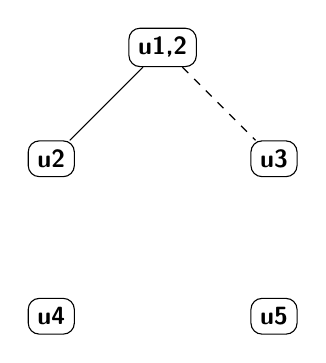
\begin{tikzpicture}[node distance=2cm,node/.style={rounded corners,draw,font=\sffamily\small\bfseries}]
	\node[node] (1) {u1,2};
	\node[node] (2)[below left of=1] {u2};
		\node[node] (3)[below right of=1] {u3};
		\node[node] (4)[below  of=2] {u4};
			\node[node] (5)[below of=3] {u5};
	\path
	(1) edge[] node [] {} (2)
		edge[dashed] node []{} (3);							
\end{tikzpicture}
\\\textbf{Step 4}
\end{minipage}
\begin{minipage}{.3\textwidth}
	 \centering
	 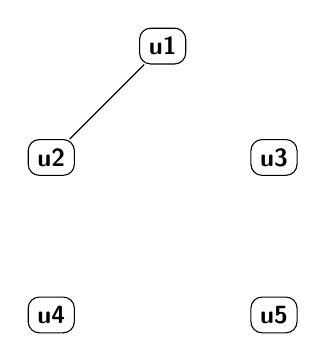
\begin{tikzpicture}[node distance=2cm,node/.style={rounded corners,draw,font=\sffamily\small\bfseries}]
	\node[node] (1) {u1};
	\node[node] (2)[below left of=1] {u2};
		\node[node] (3)[below right of=1] {u3};
		\node[node] (4)[below  of=2] {u4};
			\node[node] (5)[below of=3] {u5};
	\path
	(1) edge[] node [] {} (2);						
\end{tikzpicture}
\\ \textbf{Step 5}
\end{minipage}
\end{figure}
\end{frame}

\begin{frame}
\frametitle{Adding Edge in Data Graph }
\begin{algorithm}[H]
\caption{Dynamic data edge addition of thread t}
\textbf{Input}: Data Graph $D$,Query Graph $Q$,Delete u-v(u is parent of v).\\
\textbf{Output}: CVS updates.
\begin{algorithmic}
 \item \begin{enumerate}
 \item w=v (for u also)
\item for each child of w(till $|Q|$ length)
\begin{enumerate}
\item if acquire locks for all child of w 
\item for each NEC's x
\item C(x)=$FindCandidates$(x,D) update
\item Release all locks
\end{enumerate}
\end{enumerate}
\end{algorithmic}
\end{algorithm}
\end{frame}

\begin{frame}
\frametitle{Adding Edge in Data Graph }
\begin{figure}[h!]
\begin{minipage}{.4\textwidth}
	\centering
	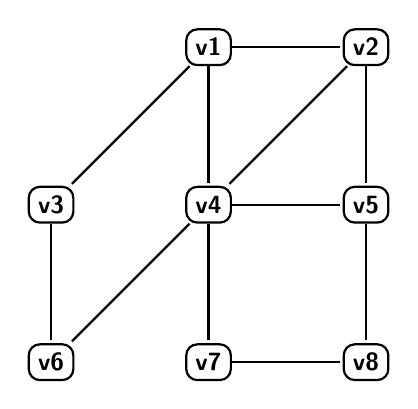
\begin{tikzpicture}[shorten >=1pt,auto,node distance=2cm,
                    thick,main node/.style={rounded corners,draw,font=\sffamily\small\bfseries}]

  \node[main node] (1) {v1};
  \node[main node] (2) [right of=1] {v2}; 
  \node[main node] (4) [below of =1] {v4};
  \node[main node] (3) [left of=4] {v3};
     \node[main node] (5) [below of=2] {v5};
    \node[main node] (6) [below of=3] {v6};
    \node[main node] (7) [below of=4] {v7};
\node[main node] (8) [below of=5] {v8};
  \path[every node/.style={font=\sffamily\small}]
    (1) edge[] node [] {} (2)
        edge[] node[] {} (3)
        edge[] node[] {} (4)
    (2) edge[] node [] {} (4)
        edge node [] {} (5)
    (3) edge[] node [] {} (6)
    (4) edge node [] {} (7)
    	edge[] node [] {} (6) 
    	edge node [] {} (5) 
    (5) edge node [] {} (8)
    (7) edge node [] {} (8);	   
\end{tikzpicture}
\\\textbf{Step 1}
\end{minipage}
\begin{minipage}{.4\textwidth}
	\centering
	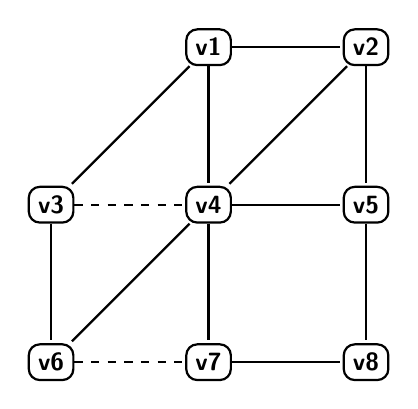
\begin{tikzpicture}[shorten >=1pt,auto,node distance=2cm,
                    thick,main node/.style={rounded corners,draw,font=\sffamily\small\bfseries}]

  \node[main node] (1) {v1};
  \node[main node] (2) [right of=1] {v2}; 
  \node[main node] (4) [below of =1] {v4};
  \node[main node] (3) [left of=4] {v3};
     \node[main node] (5) [below of=2] {v5};
    \node[main node] (6) [below of=3] {v6};
    \node[main node] (7) [below of=4] {v7};
\node[main node] (8) [below of=5] {v8};
  \path[every node/.style={font=\sffamily\small}]
    (1) edge[] node [] {} (2)
        edge[] node[] {} (3)
        edge[] node[] {} (4)
    (2) edge[] node [] {} (4)
        edge node [] {} (5)
    (3) edge[] node [] {} (6)
    	edge[dashed] node []{} (4)
    (4) edge node [] {} (7)
    	edge[] node [] {} (6) 
    	edge node [] {} (5) 
    (5) edge node [] {} (8)
    (6) edge[dashed] node[] {} (7)
    (7) edge node [] {} (8);	   
\end{tikzpicture}
\\\textbf{Step 2}
\end{minipage}
\end{figure}
\end{frame}
\begin{frame}
\frametitle{Adding Edge in Data Graph }
\begin{figure}[h!]
\begin{minipage}{.4\textwidth}
	\centering
	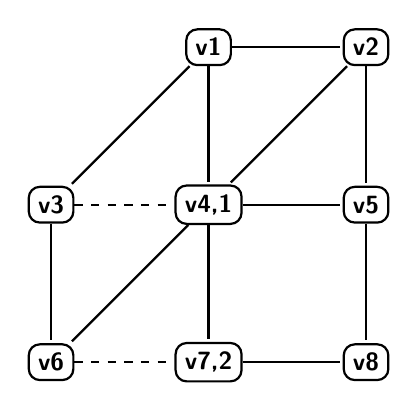
\begin{tikzpicture}[shorten >=1pt,auto,node distance=2cm,
                    thick,main node/.style={rounded corners,draw,font=\sffamily\small\bfseries}]

   \node[main node] (1) {v1};
  \node[main node] (2) [right of=1] {v2}; 
  \node[main node] (4) [below of =1] {v4,1};
  \node[main node] (3) [left of=4] {v3};
     \node[main node] (5) [below of=2] {v5};
    \node[main node] (6) [below of=3] {v6};
    \node[main node] (7) [below of=4] {v7,2};
\node[main node] (8) [below of=5] {v8};
  \path[every node/.style={font=\sffamily\small}]
    (1) edge[] node [] {} (2)
        edge[] node[] {} (3)
        edge[] node[] {} (4)
    (2) edge[] node [] {} (4)
        edge node [] {} (5)
    (3) edge[] node [] {} (6)
    	edge[dashed] node []{} (4)
    (4) edge node [] {} (7)
    	edge[] node [] {} (6) 
    	edge node [] {} (5) 
    (5) edge node [] {} (8)
    (6) edge[dashed] node[] {} (7)
    (7) edge node [] {} (8);	   
\end{tikzpicture}
\\\textbf{Step 3}
\end{minipage}
\begin{minipage}{.4\textwidth}
	\centering
	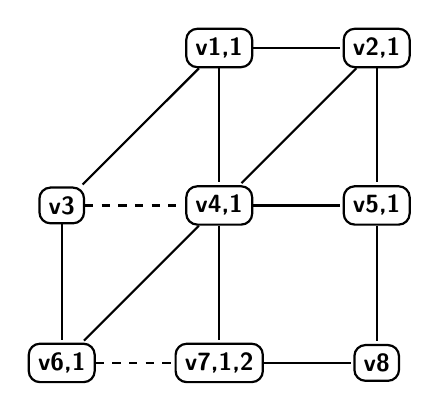
\begin{tikzpicture}[shorten >=1pt,auto,node distance=2cm,
                    thick,main node/.style={rounded corners,draw,font=\sffamily\small\bfseries}]

  \node[main node] (1) {v1,1};
  \node[main node] (2) [right of=1] {v2,1}; 
  \node[main node] (4) [below of =1] {v4,1};
  \node[main node] (3) [left of=4] {v3};
     \node[main node] (5) [below of=2] {v5,1};
    \node[main node] (6) [below of=3] {v6,1};
    \node[main node] (7) [below of=4] {v7,1,2};
\node[main node] (8) [below of=5] {v8};
  \path[every node/.style={font=\sffamily\small}]
    (1) edge[] node [] {} (2)
        edge[] node[] {} (3)
        edge[] node[] {} (4)
    (2) edge[] node [] {} (4)
        edge node [] {} (5)
    (3) edge[] node [] {} (6)
    	edge[dashed] node []{} (4)
    (4) edge node [] {} (7)
    	edge[] node [] {} (6) 
    	edge node [] {} (5) 
    (5) edge node [] {} (8)
    (6) edge[dashed] node[] {} (7)
    (7) edge node [] {} (8);	   
\end{tikzpicture}
\\\textbf{Step 4}
\end{minipage}
\end{figure}
\end{frame}
\begin{frame}
\frametitle{Adding Edge in Data Graph }
\begin{figure}[h!]
\begin{minipage}{.4\textwidth}
	\centering
	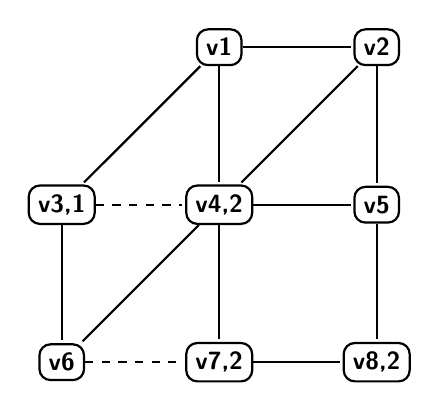
\begin{tikzpicture}[shorten >=1pt,auto,node distance=2cm,
                    thick,main node/.style={rounded corners,draw,font=\sffamily\small\bfseries}]

  \node[main node] (1) {v1};
  \node[main node] (2) [right of=1] {v2}; 
  \node[main node] (4) [below of =1] {v4,2};
  \node[main node] (3) [left of=4] {v3,1};
     \node[main node] (5) [below of=2] {v5};
    \node[main node] (6) [below of=3] {v6};
    \node[main node] (7) [below of=4] {v7,2};
\node[main node] (8) [below of=5] {v8,2};
  \path[every node/.style={font=\sffamily\small}]
    (1) edge[] node [] {} (2)
        edge[] node[] {} (3)
        edge[] node[] {} (4)
    (2) edge[] node [] {} (4)
        edge node [] {} (5)
    (3) edge[] node [] {} (6)
    	edge[dashed] node []{} (4)
    (4) edge node [] {} (7)
    	edge[] node [] {} (6) 
    	edge node [] {} (5) 
    (5) edge node [] {} (8)
    (6) edge[dashed] node[] {} (7)
    (7) edge node [] {} (8);	   
\end{tikzpicture}
\\\textbf{Step 5}
\end{minipage}
\begin{minipage}{.4\textwidth}
	\centering
	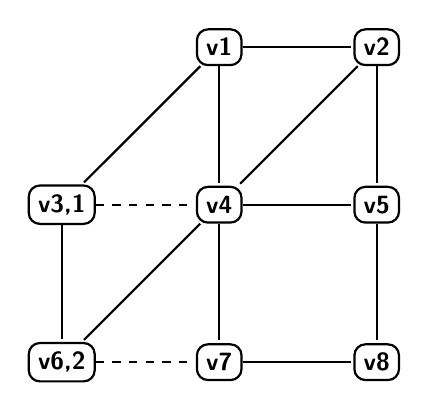
\begin{tikzpicture}[shorten >=1pt,auto,node distance=2cm,
                    thick,main node/.style={rounded corners,draw,font=\sffamily\small\bfseries}]

  \node[main node] (1) {v1};
  \node[main node] (2) [right of=1] {v2}; 
  \node[main node] (4) [below of =1] {v4};
  \node[main node] (3) [left of=4] {v3,1};
     \node[main node] (5) [below of=2] {v5};
    \node[main node] (6) [below of=3] {v6,2};
    \node[main node] (7) [below of=4] {v7};
\node[main node] (8) [below of=5] {v8};
  \path[every node/.style={font=\sffamily\small}]
    (1) edge[] node [] {} (2)
        edge[] node[] {} (3)
        edge[] node[] {} (4)
    (2) edge[] node [] {} (4)
        edge node [] {} (5)
    (3) edge[] node [] {} (6)
    	edge[dashed] node []{} (4)
    (4) edge node [] {} (7)
    	edge[] node [] {} (6) 
    	edge node [] {} (5) 
    (5) edge node [] {} (8)
    (6) edge[dashed] node[] {} (7)
    (7) edge node [] {} (8);	   
\end{tikzpicture}
\\\textbf{Step 6}
\end{minipage}
\end{figure}
\end{frame}

\begin{frame}
\frametitle{Parallel Execution }
\begin{block}{How??}
\begin{enumerate}
\item Trivial cases are working on D
\item Other cases are working on A and B
\end{enumerate}

\end{block}
\end{frame}


\begin{frame}
\frametitle{Conclusion }
\begin{block}{Conclusion}
\begin{enumerate}
\item We studied the Sub-graph Isomorphism problem and the state-of-art algorithms. We came to know they are using different pruning techniques to avoid the false candidates as early as possible. 
\item FindTreeMatch should be run at each output stage which is the costlier of all stages. Running a subgraph isomorphism solution after applying all edge updates becomes equally fast as the dynamic version
\end{enumerate}

\end{block}
\end{frame}

%\begin{frame}{Future work}
%\begin{block}{}
%\begin{enumerate}
%\item Using clique to clique edges\\
%\hspace{10mm} This will help to reduce the amount of search since clique has all the subgraphs.
%\item Using multiple trees to create CVS\\
%\hspace{10mm} We can use multiple trees to create the unique numbering so %that it will reduce the candidate set size.
%\item Multiple Query Graphs\\
%\hspace{10mm} Processing for multiple query graphs simultaneously.
%\item Dynamic Queries\\
%\hspace{10mm} The query graph and data graph can change. So we update the previous answers accordingly.
%\end{enumerate}
%\end{block}

%\end{frame}



\begin{frame}
	
\color{violet} \Huge{\centerline{Thank You}}
\end{frame}

\end{document} 